\chapter{Materiais e Métodos}

O ETHEL foi originalmente desenvolvido utilizando Python 3 e as bibliotecas \textit{bluetooth}, \textit{cwiid}, \textit{datetime}, \textit{math}, \textit{numpy}, \textit{os}, \textit{pyGTk}, \textit{sys}, \textit{xlrd}, \textit{xlwt} e \textit{xlutils} (\citeauthor{Thales2018}, \citeyear{Thales2018}). As versões das bibliotecas utilizadas atualmente no ETHEL são elencadas na \textbf{Tabela \ref{modulosETHEL}}. 

% Please add the following required packages to your document preamble:
% \usepackage{booktabs}
\begin{table}[]
\caption{Módulos  presentes no atualmente ETHEL, executados com a versão 3.6.8 do Python}
\label{modulosETHEL}
\centering
\begin{tabular}{@{}ll@{}}
\toprule
\textbf{Biblioteca} & \multicolumn{1}{c}{\textbf{Versão}} \\ \midrule
bluetooth           & 0.22                                \\
cwiid               & 3.0.0                               \\
datetime            & 4.3                                 \\
math                & 3.5                                 \\
matplotlib          & 3.0.3                               \\
numpy               & 1.16.3                              \\
os                  & 3.2                                 \\
pyGTK               & 3.0                                 \\
pygame              & 1.9.5                               \\
sqllite3            & 2.0                                 \\ \bottomrule
\end{tabular}
\end{table}

As novas métricas (cálculo da excursão máxima AP e ML e módulo LOS) foram desenvolvidas e incluídas na nova versão do ETHEL. Para implementar o LOS foi utilizada a biblioteca \textit{pygame}, que é uma  biblioteca usada na criação de aplicações multimídia como jogos. A \textit{pygame} foi escolhida por atender as necessidades para o  desenvolvimento do LOS e por ser uma biblioteca bastante documentada. Além disso, ela é altamente portável e roda em praticamente todas plataformas e sistemas operacionais. 

Na próxima seção são apresentados maiores detalhes sobre estas implementações.

\section{Desenvolvimento de novas métricas no ETHEL}

O ETHEL é um sistema de avaliação do equilíbrio corporal que utiliza a WBB como plataforma de força para estimar as métricas necessárias na avaliação do equilíbrio. Ele permite capturar os sinais gerados pela WBB (utilizando a tecnologia \textit{bluetooth}), calcula e apresenta os parâmetros quantitativos utilizados na posturografia.  

Os parâmetros são calculados no ETHEL com base no COP, são os valores de deslocamento ântero-posterior (AP) e deslocamento médio-lateral (ML). A partir desses valores são calculados outras métricas como : \textit{totex} (somatório das distâncias entre os valores do COP), \textit{totexParcial}  (somatório das distâncias entre os valores no eixo x (ML) e no eixo y (AP)), distância média (do COP), distância resultante (do COP), distância média quadrática (do COP) e a velocidade média (\textit{totex}/tempo) (\citeauthor{Thales2018}, \citeyear{Thales2018}).

Para viabilizar a proposta de validação, se fez necessário a implementação de algumas métricas no ETHEL que estão presentes no \textit{Posturography Test}. 
As novas métricas que foram implementadas são: a excursão máxima nos eixos médio-lateral (ML) e ântero-posterior (AP). A velocidade média que também é uma métrica estimada no \textit{Posturography Test} e, já estava implementada no ETHEL. Para estimar a média das métricas implementadas é necessário realizar três repetições das quatro condições sensoriais (olhos abertos em uma superfície plana, olhos fechados em uma superfície plana, olhos abertos sobre espuma e olhos fechado sobre espuma) descritas no mCTSIB  que é uma versão simplificada do Teste de Organização Sensorial (\citeauthor{ford1995test}, \citeyear{ford1995test}).

A excursão máxima é o intervalo de maior distância entre dois pontos do deslocamento do COP, na direção AP e ML. Este intervalo pode ser calculado como o valor absoluto da diferença entre o maior valor e o menor valor nas respectivas séries temporais. Quando o intervalo é calculado no eixo x estima-se a Excursão Máxima ML e quando calculado no eixo y estima-se  a Excursão Máxima AP (\citeauthor{prieto1996measures}, \citeyear{prieto1996measures}). 


O módulo do LOS também foi implementado no ETHEL. O LOS é um teste dinâmico de equilíbrio, ele mensura a variação do COP do indivíduo submetido a estímulos em diferentes direções, dentro da sua base de apoio sem alterá-la, e avalia sua capacidade de manter brevemente sua estabilidade nessas posições. Para realização do LOS computadorizado, são geradas oito posições de destino, a tarefa do paciente é se mover na direção da posição (selecionada aleatoriamente das oito posições geradas) indicada no momento, dentro da sua base suporte e sem mover seus pés. No LOS três medidas são apresentadas como resultado: tempo de reação, excursão máxima e controle direcional. O tempo de reação que é definido como o tempo entre a indicação visual do alvo e o inicio do deslocamento do centro de massa do participante na direção do alvo. A excursão máxima é a distância máxima que o participante pode deslocar seu COP na direção indicada, sem alterar sua base de apoio. O controle direcional é avaliado como a porcentagem de movimento na direção do alvo em relação ao movimento total pretendido (no alvo) (\citeauthor{tsang2003effects}, \citeyear{tsang2003effects}), (\citeauthor{llorens2015low}, \citeyear{llorens2015low}).

\section{Testes}
Para avaliar a viabilidade da metodologia proposta e testar as novas métricas implementadas no ETHEL foram realizados testes com voluntários entre os dias 2 e 7 de agosto de 2019, pela equipe do projeto "Validação do Sistema ETHEL para avaliação do equilíbrio corporal" (\textbf{Anexo \ref{anexoCEP}}). Os resultados foram cedidos ao presente trabalho. Nove adultos saudáveis, com idades entre 20 e 50 anos, participaram dos testes com o ETHEL (sexo = 7 homens e 2 mulheres). Nenhum dos participantes relatou alguma doença ou uso de medicação que pudesse influenciar no controle do equilíbrio. Ademais, foram avaliados por uma fisioterapeuta. O estudo foi aprovado pelo CEP da UESC e todos assinaram um termo de consentimento, onde foram informados dos objetivos da pesquisa. 

Na realização dos teste com o ETHEL a WBB foi utilizada como plataforma de força. Um notebook
com o processador Intel® Core™ i5-4210U CPU @ 1.70GHz, 8 GB de RAM e placa de vídeo \textit{NVIDIA Corporation Geforce} 610M e conexão \textit{bluetooth} 4.1 foi utilizado na aquisição dos dados. No entanto, os requisitos mínimos para utilização do software ETHEL é um computador que tenha tecnologia \textit{bluetooth} e que tenha como sistema operacional uma distribuição \textit{Unix}.

A coleta dos dados foi supervisionada por uma fisioterapeuta experiente, a qual instruiu os participantes sobre a realização dos testes. Durante os testes, os participantes permaneceram imóveis por 30 segundos sobre a WBB em quatro condições sensoriais diferentes: olhos abertos em uma superfície plana (OASP), olhos fechados em uma superfície plana (OFSP), olhos abertos sobre a espuma (OASE) e olhos fechados sobre a espuma (OFSE) (\textbf{Figura \ref{mctsib}}). Três repetições de cada condição foram realizadas para estimar a velocidade média e a média da excursão máxima nos eixos médio-lateral (ML) e ântero-posterior (PA). Uma pausa de 10 segundos foi concedida aos participantes entre cada repetição. É importante ressaltar que, para cada paciente, foi utilizada a mesma WBB como plataforma de força.

\begin{figure}[ht]
\captionsetup{justification   = raggedright,
              singlelinecheck = false}
\caption{Condições Sensoriais}\label{mctsib}
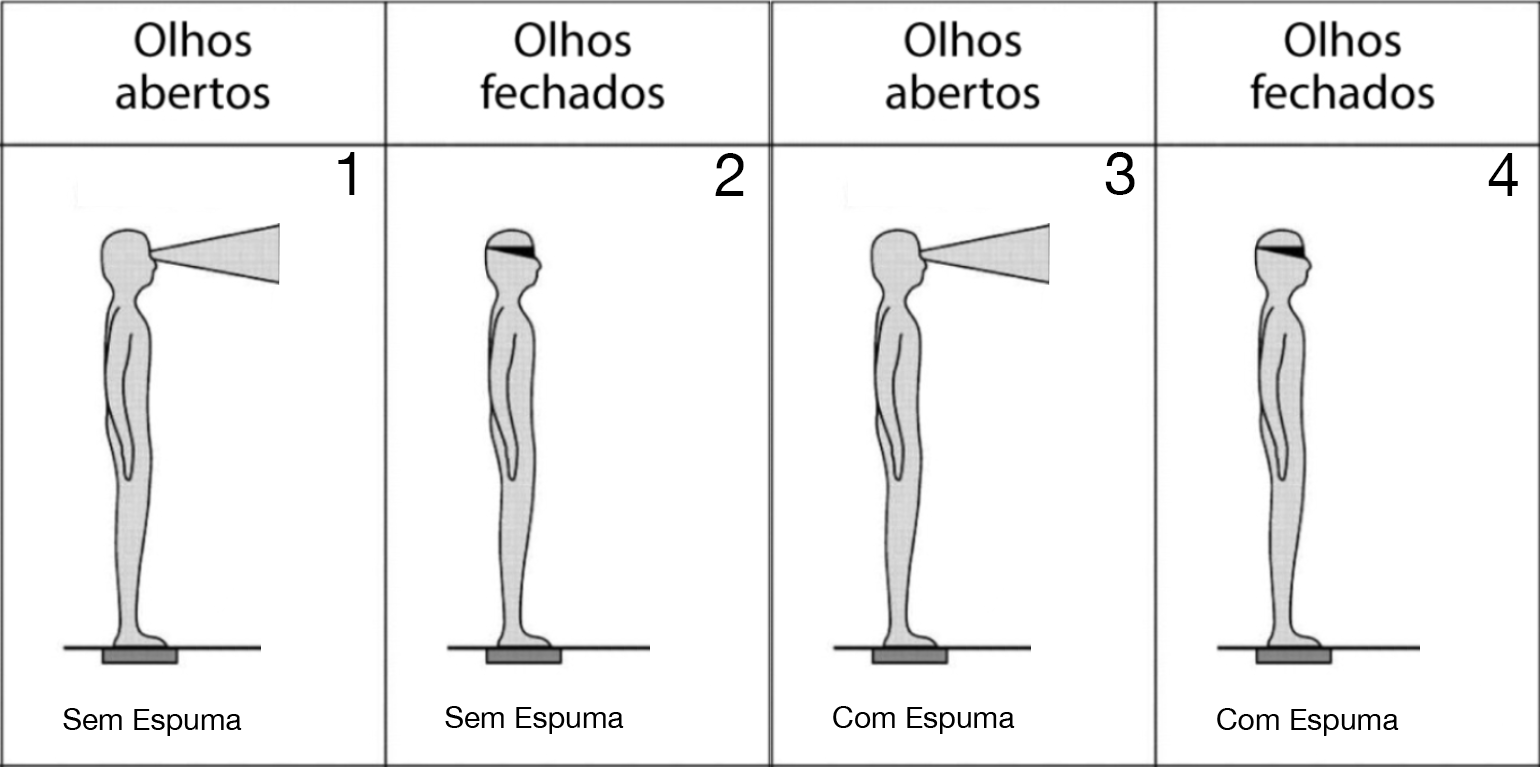
\includegraphics[width=1.0\textwidth]{mctsib.png}
\end{figure}


Ao fim dos testes, foi calculado o desvio padrão que é uma medida que  expressa o grau de dispersão de um conjunto de dados. E o erro relativo, que mostra o desvio da primeira repetição em relação a média das três repetições.